\documentclass[xcolor=dvipsnames]{beamer}
\usepackage{beamerthemelined}
\usepackage{pstricks}
\usepackage{animate}
\usepackage{graphicx}

\setbeamertemplate{navigation symbols}{}
\usepackage{caption}
\captionsetup{textfont={small,bf,color=cyan}}
\captionsetup{labelformat=empty}

\usepackage{ifthen,xifthen}
\newenvironment{items}[1][]
{\begin{itemize}
    \ifthenelse{\isempty{#1}}
    {\setlength{\itemsep}{12pt}}{\setlength{\itemsep}{#1}}}
  {\end{itemize}}

%%% Standard math:
\usepackage{amsfonts,amssymb,amsmath,amsthm} % Math packages
\newcommand{\st}{\displaystyle} % For making small math big
\renewcommand{\t}{\text} % For text in math environment
\renewcommand{\c}{\cdot} % Multiplication dot in math
\newcommand{\f}[2]{\dfrac{#1}{#2}} % Shortcut for fractions
\newcommand{\p}[1]{\left(#1\right)} % Parenthesis
\renewcommand{\sp}[1]{\left[#1\right]} % Square parenthesis
\newcommand{\set}[1]{\left\{#1\right\}} % Curly parenthesis
\newcommand{\abs}[1]{\left|#1\right|} % Absolute value

%%% Physics symbols, vectors
\let\vepsilon\epsilon
\let\vphi\phi
\renewcommand{\epsilon}{\varepsilon} % Prettier epsilon
\renewcommand{\phi}{\varphi} % Prettier phi
\renewcommand{\l}{\ell} % Prettier l
\renewcommand{\v}[1]{\boldsymbol{\mathrm{#1}}} % Bold vectors
\newcommand{\uv}[1]{\hat{\boldsymbol{\mathrm{#1}}}} % Unit vectors
\newcommand{\del}{\v\nabla} % Del operator
\renewcommand{\d}{\partial} % Partial d
\newcommand{\fd}[2]{\f{d #1}{d #2}} % First derivative
\newcommand{\sd}[2]{\f{d^2 #1}{d^2 #2}} % Second derivative
\newcommand{\fpd}[2]{\f{\d #1}{\d #2}} % First partial derivative
\newcommand{\spd}[2]{\f{\d^2 #1}{\d^2 #2}} % Second partial derivative
\newcommand{\cxv}[1]{\v{\widetilde{#1}}} % Complex variable

\title{Investigating an Optical Vortex (THIS BEGS FOR A NEW TITLE!!!111!!!@!@!!!!)}
\author{Aaron Kratzer, David Grant, Paho Lurie-Gregg,
  Michael Perlin, Grant Sherer}
\date{06 December 2013}

\begin{document}

\begin{frame}
  \maketitle
\end{frame}

\begin{frame}
	\frametitle{Generation - Multilayer Spiral Phase Plate}
  \begin{columns}[c]
    \column{0.6\textwidth}
    \begin{items}
    \item SiO$_2$ is deposited onto a substrate using an electron beam
    \item Since the plate thickness varies with $\phi$, the phase
      develops the $\phi$ dependence that produces a helical wave
      front
    \end{items}
    \column{0.4\textwidth}
    \begin{figure}
      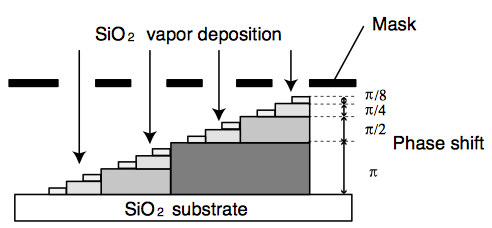
\includegraphics[width=\columnwidth]{MSPP.jpg}
      \caption{SiO$_2$ Phase Plate}
      \label{MSPP}
    \end{figure}
  \end{columns}
\end{frame}

\begin{frame}
	\frametitle{Generation - Computer Generated Holography}
  \begin{items}
  \item A reference wave and a particular object wave are combined to
    form an interference pattern.
  \item The interference pattern is then produced as a hologram
    filament.
  \item When a beam propagates through this filament, the first order
    diffraction beam contains the optical vortex.
  \end{items}
\end{frame}

\begin{frame}
	\frametitle{Application: Twisted Radio Waves}
	\begin{center}
		\emph{Single frequency, multiple channel encoding via vorticity}
	\end{center}
  \begin{columns}[c]
    \column{0.5\textwidth}
    \begin{figure}
      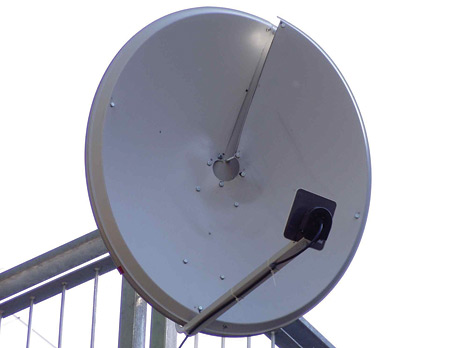
\includegraphics[width=\textwidth]{helical_dish}
      \caption{A helical dish transmitter designed for the $\ell=1$
        mode}
      \label{pic:dish}
    \end{figure}
    \column{0.5\textwidth}
		\begin{items}
		\item First test in radio spectrum
		\item Public far field test
		\item Multiple radio signals transmitted on the same frequency
		\end{items}
	\end{columns}
\end{frame}

\begin{frame}
	\frametitle{Experimental Setup}
  \begin{columns}{c}
    \column{0.5\textwidth}
		\begin{figure}
      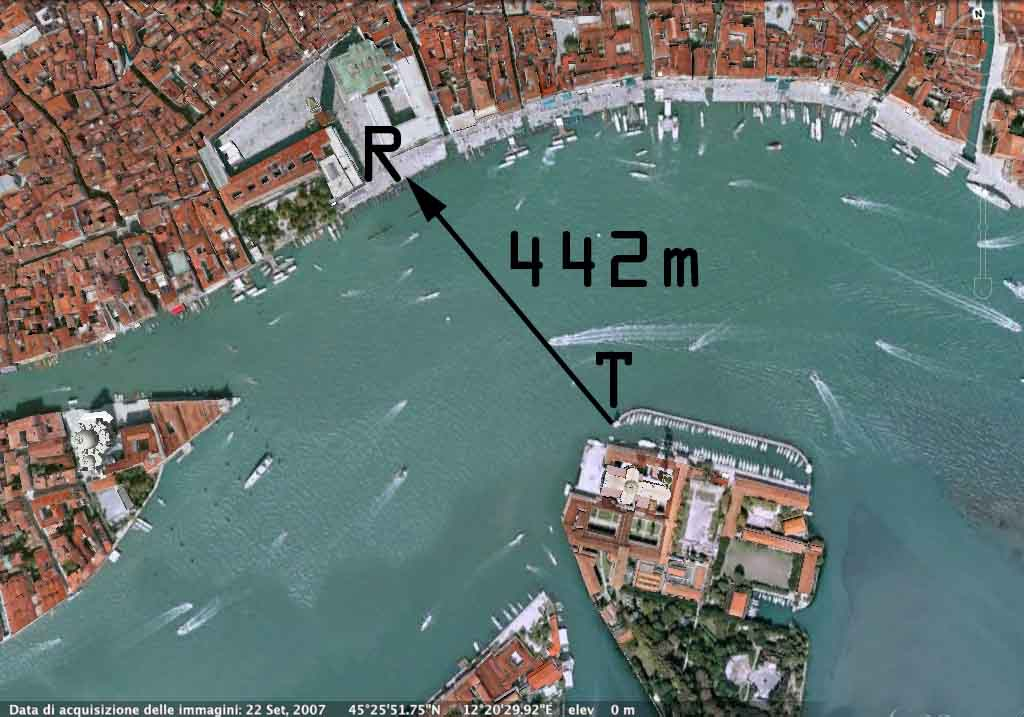
\includegraphics[width=\textwidth]{birdeyeview}
      \caption{Transmission path}
      \label{pic:birdeye}
		\end{figure}
    \column{0.5\textwidth}
		\begin{items}
		\item Transmitted distance $\gg$ radio wavelength
		\item Transmitted at 2.414 GHz, $\Delta \nu = 15MHz$
		\item 
		\end{items}
  \end{columns}
\end{frame}

\begin{frame}
  \begin{columns}{c}
    \column{0.5\textwidth}
		\begin{figure}
      %\includegraphics[width=\textwidth]{}
      \caption{}
      \label{}
		\end{figure}
    \column{0.5\textwidth}
		\begin{items}
		\item Real world senario
		\item Vorticity preserved
		\end{items}
  \end{columns}

Same carrier frequency (2.4GHz), 440 Hz and 1000 Hz audio signals were transmitted via the planar and twisted wave, respectively.
\end{frame}

\begin{frame}
  \frametitle{Vector potential}
  \begin{align*}
    {\cxv A}\p{r,\phi,z}&=A_0\f{w_0}{w}\sp{\f{r\sqrt 2}{w}}^\ell
    L^{\p{\ell}}_p\sp{2\f{r^2}{w^2}}\exp\sp{-\f{r^2}{w^2}} \\
    &~~~\times\exp\sp{-i\f{kr^2z}{2\p{z^2+z_R^2}}}
    \exp\sp{i\p{2p+\ell+1}\arctan\p{\f z{z_R}}} \\
    &~~~\times\exp\p{i\ell\phi}\exp\p{-i\omega t} \uv r \\
    L^{\p{\ell}}_p\p{x}
    &=\sum_{m=0}^p\p{-1}^m\f{\p{p+\ell}!}{\p{p-m}!\p{\ell+m}!m!}x^m \\
    L^{\p{3}}_1\p{x}&=-x+4
  \end{align*}
\end{frame}

\begin{frame}
  \frametitle{Physical fields}
  \begin{align*}
    \cxv E&=i\omega\cxv A \\
    \cxv B&=\del \times\cxv A \\
    &={\varepsilon^i}_{jk}\uv e_i\d^jA^k \\
    &={\varepsilon^i}_{jk}\uv
    e_i\sp{A^k\p{x^j+\delta}-A^k\p{x^j}}/\delta \\
    \v S&=\v E\times\v H \\
    u&=\f12\p{\v E\c\v D+\v B\c\v H} \\
    I&=\f c2\v E\c\v D
  \end{align*}
\end{frame}

\begin{frame}
  \frametitle{Force per unit volume}
  \begin{align*}
    \sigma^{ij}&=\epsilon\p{E^iE^j-\f12\delta^i_j\abs{\v E}^2}
    +\f1\mu\p{B^iB^j-\f12\delta^i_j\abs{\v B}^2} \\
    \v f&=\del\c\sigma-\d_t\v S/c^2 \\
    &=\p{\d^k\sigma^{ik}-\d_tS^i/c^2}\uv e_i
  \end{align*}
\end{frame}

% Animation bullshit
\begin{frame}
  \frametitle{Electric Field}
  \begin{columns}[T,totalwidth=\textwidth]
    \column{.5\textwidth}
    \begin{figure}[h]
      \centering \animategraphics[width=1.15\columnwidth, loop,
      autoplay] {5}{anim/slice-Ex-}{00}{29}
    \end{figure}

    \column{.5\textwidth}
    \begin{figure}[h]
      \centering \vspace{-.6in} \animategraphics[width=.8\columnwidth,
      loop, autoplay] {5}{anim/3d-E-}{00}{29}
    \end{figure}

  \end{columns}
\end{frame}

\begin{frame}
  \frametitle{Magnetic Field}
  \begin{columns}[T,totalwidth=\textwidth]
    \column{.5\textwidth} \vspace{-.3in}
    \begin{figure}[h]
      \centering \animategraphics[width=.85\columnwidth, loop,
      autoplay] {5}{anim/slice-By-}{00}{29}
      \animategraphics[width=.85\columnwidth, loop, autoplay]
      {5}{anim/slice-Bz-}{00}{29}
    \end{figure}

    \column{.5\textwidth}
    \begin{figure}[h]
      \centering \vspace{-.4in} \animategraphics[width=.8\columnwidth,
      loop, autoplay] {5}{anim/3d-B-}{00}{29}
    \end{figure}

  \end{columns}
\end{frame}

\begin{frame}
  \frametitle{Poynting Vector} \vspace{1mm}
  \begin{columns}[T,totalwidth=\textwidth]
    \column{.5\textwidth} \vspace{-.3in}
    \begin{figure}[h]
      \centering \animategraphics[width=.85\columnwidth, loop,
      autoplay] {5}{anim/slice-Sy-}{00}{29}
      \animategraphics[width=.85\columnwidth, loop, autoplay]
      {5}{anim/slice-Sz-}{00}{29}
    \end{figure}
    \column{.5\textwidth}
    \begin{figure}[h]
      \centering \vspace{-.4in} \animategraphics[width=.8\columnwidth,
      loop, autoplay] {5}{anim/3d-S-}{00}{29}
    \end{figure}

  \end{columns}
\end{frame}

\end{document}
